\documentclass[tikz,border=10pt]{standalone}
\usepackage{tikz}
\usetikzlibrary{calc}

\begin{document}
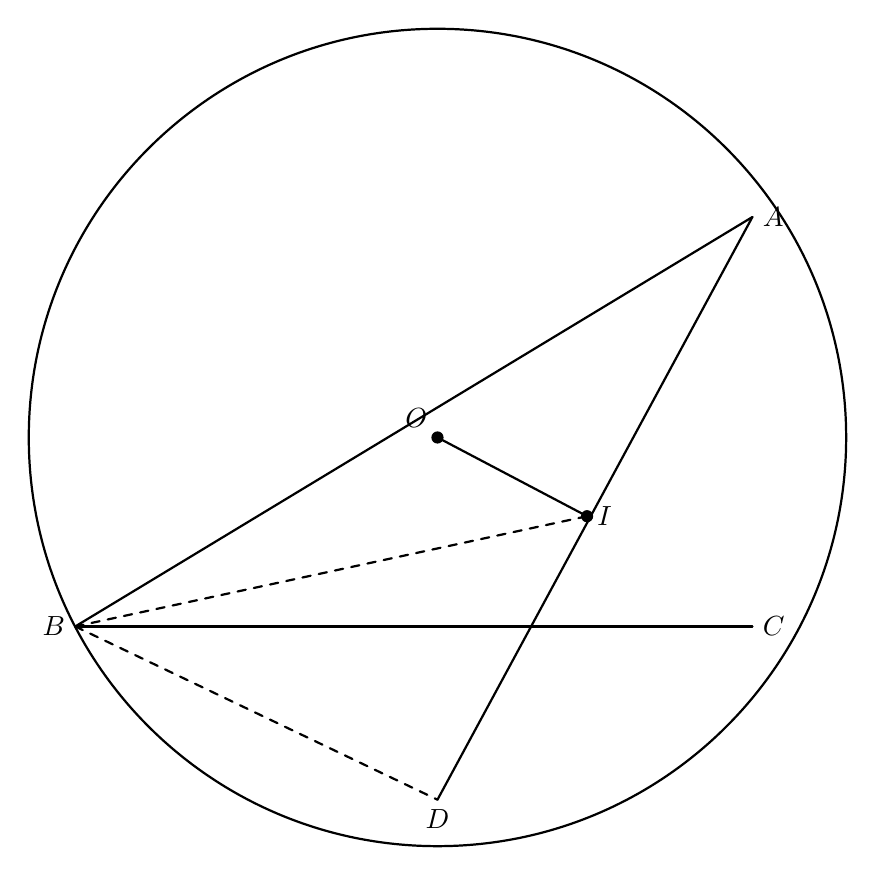
\begin{tikzpicture}[line cap=round,line join=round,thick]

% Coordinates
\coordinate (O) at (0,0);
\coordinate (B) at (-4.6,-2.4);
\coordinate (A) at (4.0,2.8);
\coordinate (C) at (4.0,-2.4);
\coordinate (D) at (0,-4.6);
\coordinate (I) at (1.9,-1.0);

% Circle radius chosen so that A,B,C,D lie on it
\def\r{5.1904}

% Circle
\draw (O) circle (\r);

% Solid segments
\draw (B) -- (A);
\draw (B) -- (C);
\draw (A) -- (D);
\draw (O) -- (I);

% Dashed segments
\draw[dashed] (B) -- (I);
\draw[dashed] (B) -- (D);

% Point markers
\fill (O) circle (2.2pt);
\fill (I) circle (2.2pt);

% Labels
\node[above left] at (O) {$O$};
\node[right] at (A) {$A$};
\node[left] at (B) {$B$};
\node[right] at (C) {$C$};
\node[below] at (D) {$D$};
\node[right] at (I) {$I$};

\end{tikzpicture}
\end{document}
